\documentclass[12pt]{article}
\linespread{1.6}

\usepackage{amssymb,amsfonts,amsmath,mathtext}
\usepackage{graphicx}
\graphicspath{{images/}}
\usepackage{indentfirst}
\usepackage{xcolor}
\usepackage{soul}
\usepackage{comment}
\usepackage{hyperref}
\hypersetup{
    colorlinks=true,
    linkcolor=black,
    filecolor=cyan,   
    urlcolor=blue,
    pdftitle={Проект 1673 Отчет №1},
    pdfpagemode=FullScreen,
    }
\usepackage[T2A]{fontenc}
\usepackage[utf8]{inputenc}
\usepackage{hyphenat}
\usepackage{cite,enumerate}
\usepackage[russian,english]{babel}
\usepackage{mathtools}
\usepackage{physics}

%\usepackage[ruled,vlined]{algorithm2e}
\usepackage{algorithm}
\usepackage{algpseudocode}

\usepackage[%
    left=2.0in,%
    right=1.0in,%
    top=2.0in,%
    bottom=2.0in,%
    %paperheight=11in,%
    %paperwidth=8.5in%
]{geometry}%

%\usepackage[document]{ragged2e}
\emergencystretch=4em

%\DeclarePairedDelimiter\abs{\lvert}{\rvert}
%\DeclarePairedDelimiter\norm{\lVert}{\rVert}

\DeclareUnicodeCharacter{2212}{\textendash} %чтоб input был корректный

% формулы нумеруются внутри каждой главы
%\numberwithin{equation}{chapter}

% Заменяем библиографию с квадратных скобок на точку:
%\makeatletter
%\renewcommand{\@biblabel}[1]{#1.} 
%\makeatother

\addtolength{\oddsidemargin}{-.5in}
\addtolength{\evensidemargin}{-.5in}
\addtolength{\textwidth}{1in}

\addtolength{\topmargin}{-.5in}
\addtolength{\textheight}{1in}

\newtheorem{definition}{Определение}
%-----------------------------------------------------------

\begin{document}
\begin{titlepage}
\begin{center}
Федеральное государственное автономное образовательное учреждение высшего образования
\\
Национальный исследовательский университет\\
«Высшая школа экономики»\\
Московский институт электроники и математики\\
Департамент прикладной математики\\
Руководитель проекта, Инициатор проекта: Байдин Георгий Сергеевич\\
Руководитель направления: Крук Евгений Аврамович\\
\vspace{24pt}
\huge Обзор основных алгоритмов постквантовой криптографии\\
\vspace{96pt}
\large Команда проекта №1673 \\
Гор Сарибекян\\
Станислав Манжилевский\\
Шамиль Валиев\\
Анастасия Простенко\\
\vspace{12pt}
%Due Date: January 1, 2023 \\
%Submitted: January 1, 2023 \\
\end{center}
\end{titlepage}

\pagenumbering{gobble}
%\section*{Abstract}

This document is provided as a \textit{template only} and is used for all reports in Unit Ops 1, 2, and 3. This means you may not need to use all parts of the template. \textbf{Refer to the Lab Report Guidelines document available on Canvas for specific guidance related to the required sections, appendices, figures, etc. for your report.} Make sure to rename sections, subsections, etc. as needed for your report.

If you recompile while viewing main.tex, all subfiles (the entire report) will be contained in the pdf.

To remove an unneeded section, simply delete the relevant \textbackslash subfile\{...\} command in main.tex.

This template uses filler text. It was inserted using the command \textbackslash lipsum[...]. Remove those commands to remove the filler text.

\clearpage
\renewcommand{\contentsname}{Содержание}
\tableofcontents
\clearpage
%\listoffigures
%\clearpage
%\listoftables %remove this line if you do not have any tables
%\clearpage

\renewcommand{\figurename}{Рисунок}

\pagenumbering{arabic}
\section{Цели работы, поставленные задачи}

Задачей данного обзора является рассмотрение наиболее перспективных направлений развития алгоритмов постквантовой криптографии и основных их представителей. В частности:



\begin{itemize}
    \item Коды, исправляющие ошибки, и криптосхема Мак-Элиса;
    \item Целочисленные решётки и криптосхема CRYSTALS-Kyber;
    \item Скрытые уравнения поля и криптосхема GeMSS;
    \item Хэш-функции и криптосхема SPHINCS$^+$
\end{itemize}

Мы выбрали данные криптоагоритмы так как они прошли 3 раунд конкурса NIST (National Institute of Standards and Technology) по выбору квантово-устойчивых криптоалгоритмов. Конкурс стартовал в 2017 году и был нацелен на выбор алгоритмов постквантовой криптографии, пригодных для выдвижения в качестве стандартов. 

Мы сосредоточимся на анализе математических основ данных алгоритмов, их применимости в различных сценариях, а также оценке эффективности их реализаций.
\clearpage
\section{Перечень сокращений и обозначений}

\textbf{AES} (Advanced Encryption Standard) -- Алгоритм симметричного шифрования

\textbf{DO} (Dembowski-Ostrom) -- Полиномы Дембовского-Острома

\textbf{DS} (Digital Signature) -- Цифровая подпись

\textbf{FORS} (Forest of Random Subsets) -- Лес случайных подмножеств

\textbf{FTS} (Few-time signature) -- Схема ограниченно-многоразовой подписи

\textbf{GeMSS} (Great Multivariate Short Signature)

\textbf{HFE} (Hidden Field Equations) -- Скрытые уравнения поля

\textbf{HFEv} (HFE with vinegar) 

\textbf{HFEv-} (HFE with vinegar and minus) 

\textbf{HQC} (Hamming Quasi-Cyclic) 

\textbf{IKE} (Internet Key Exchange) -- Протокол обмена ключами в сети Интернет

\textbf{KEM} (Key Encapsulation Mechanism) -- Механизм инкапсуляции ключа

\textbf{LWE} (Learning With Errors) -- Обучение с ошибками

\textbf{MQ} (Multivariate Quadratic) -- Задача многомерных квадратных уравнений

\textbf{MTS} (Many-time signature) -- Схема многоразовой подписи

\textbf{NIST} (National Institute of Standards and Technology) -- Национальный Институт Стандартов и Технологий

\textbf{OTS} (One-Time Signature) -- Одноразовая подпись

\textbf{SIS} (Short Integer Solution) -- Кратчайшее целочисленное решение

\textbf{SSL} (Secure Sockets Layer)

\textbf{TLS} (Transport Layer Security) -- Протокол защиты транспортного уровня

\textbf{WOTS} (Winternitz-type One-Time Signature) -- Схема одноразовой подписи Винтерница

\textbf{WOTS+} (Winternitz-type One-Time Signature) -- Модифицированная схема одноразовой подписи Винтерница

\textbf{XMSS} (eXtended Merkle Signature Scheme) 

\textbf{ЭЦП} -- Электронная цифровая подпись

\clearpage
\section{Термины и определения}

\textbf{Алгоритм зашифрования} — алгоритм криптографический, реализующий функцию зашифрования. В случае шифрсистем блочных получается использованием алгоритма зашифрования блочного базового в конкретном режиме шифрования.

\textbf{Алгоритм криптографический} — алгоритм, реализующий вычисление одной из функций криптографических.

\textbf{Алгоритм расшифрования} — алгоритм криптографический, обратный к алгоритму зашифрования и реализующий функцию расшифрования.

\textbf{Алгоритм шифрования} — под алгоритмом шифрования в зависимости от контекста понимается алгоритм зашифрования или алгоритм расшифрования.

\textbf{Анализ криптографический} — исследование системы криптографической с целью получения обоснованных оценок ее стойкости криптографической. Результаты а. к. могут использоваться разработчиком и пользователем законным криптосистемы для оценки эффективности системы защиты информации от потенциального противника и/или нарушителя, а потенциальным противником и/или нарушителем для подготовки и реализации атаки на криптосистему. А. к. проводится путем исследования криптосистемы, а также моделирования (выполнения) различных атак на криптосистему.

\textbf{Аутентификация сообщения} — проверка того, что сообщение было получено неповрежденным, неизмененным (с момента отправления), то есть проверка целостности. Если стороны доверяют друг другу, то а. с. осуществляется применением системы имитозащиты. Для не доверяющих друг другу сторон необходимо использовать систему подписи цифровой.

\textbf {Дешифрование} — процесс аналитического раскрытия противником и/или нарушителем сообщения открытого без предварительного полного знания всех элементов системы криптографической. Если этот процесс поддается математической формализации, говорят об алгоритме дешифрования.

\textbf{Система криптографическая} — система обеспечения безопасности информации криптографическими методами в части конфиденциальности, целостности, аутентификации, невозможности отказа и неотслеживаемости. В качестве подсистем может включать системы шифрования, системы идентификации, системы имитозащиты, системы подписи цифровой и др., а также систему ключевую, обеспечивающую работу остальных систем. В основе выбора и построения с. к. лежит условие обеспечения стойкости криптографической.

\textbf{Хеш-значение (hash-code)} —значение хеш-функции для данного аргумента.

\textbf{Хеш-функция} — функция, отображающая входное слово конечной длины в конечном алфавите в слово заданной, обычно фиксированной длины.

\textbf{Хеш-функция криптографическая}  — хеш-функция, сочетающая в себе свойства хеш-функции односторонней, хеш-функции с прообразами вторыми трудно обнаружимыми и хеш-функции с коллизиями трудно обнаружимыми. Особо выделяют хеш-функции криптографические, задаваемые ключом, имеющие другое содержание.

\clearpage

\section{Вступление}
В настоящее время абсолютное большинство информационных систем передачи данных используют на одном из этапов шифрования асимметричные криптосистемы с открытым ключом. Большой проблемой такого подхода является уязвимость современных алгоритмов асимметричного шифрования в обозримом будущем.

По оценками специалистов компании QApp \cite{quantumthreat}, к 2028 году возможно появление достаточно мощного квантового компьютера для реализации на нём алгоритма Шора \cite{Shor} и решения задач факторизации и дискретного логарифмирования, лежащих в основе используемых на данный момент криптосистем, используемых в таких протоколах шифрования данных в сети, как TLS или IKE.

В связи с возрастающей угрозой необходимо уже сейчас использовать для передачи данных криптографические алгоритмы достаточно стойкие, чтобы в перспективе противостоять криптоанализу с применением квантового компьютера. В данной статье приведён обзор наиболее перспективных направлений развития постквантовой криптографии и описаны их представители.

\clearpage

\section{Выполнение работы}
\subsection{Критерии сравнения}
Могут быть выделены следующие критерии сравнения соответствующих алгоритмов:

\subsubsection{Тип криптографического алгоритма}
Как было показано выше, существует большое разнообразие типов криптографических алгоритмов. При выборе какого-то из них для тех или иных целей необходимо учитывать математические аспекты его реализации, потому что вопрос о надёжности математической базы является дискуссионным\cite{lattice_attack}, и по причине постоянного развития в сфере криптоанализа нельзя с полной уверенностью утверждать, что какая либо из криптосистем не будет скомпрометирована в дальнейшем.

\subsubsection{Заявляемая стойкость криптографического примитива/реальная стойкость криптографического примитива}

Для оценки качественных свойств криптографических свойств алгоритмов, NIST ввёл несколько уровней стойкости по критерию количества вычислительных ресурсов, необходимых для поиска ключа, с аналогичной характеристикой для указанной в уровне симметричной криптосистемой\cite{Security_Evaluation_Criteria}:
\begin{enumerate}
    \item Любая атака, соответствующая 1-у уровню безопасности, должна требовать вычислительных ресурсов, сравнимых или превышающих те, которые требуются для поиска ключа в блочном шифре со 128-битным ключом (например, AES128).
    \item Любая атака, соответствующая 2-у уровню безопасности, должна требовать вычислительных ресурсов, сравнимых или превышающих те, которые требуются для поиска коллизий в 256-битовой хэш-функции (например, SHA256/ SHA3-256).
    \item Любая атака, соответствующая 3-у уровню безопасности, должна требовать вычислительных ресурсов, сравнимых или превышающих те, которые требуются для поиска ключа в блочном шифре со 192-битным ключом (например, AES192).
    \item Любая атака, соответствующая 4-у уровню безопасности, должна требовать вычислительных ресурсов, сравнимых или превышающих те, которые требуются для поиска коллизий в 384-битовой хэш-функции (например, SHA384/ SHA3-384).
    \item Любая атака, соответствующая 5-у уровню безопасности, должна требовать вычислительных ресурсов, сравнимых или превышающих те, которые требуются для поиска ключа в блочном шифре с 256-битным ключом (например, AES 256).
\end{enumerate}

В настоящий момент в качестве эквивалента для сравнения уровня стойкости криптографических алгоритмов используют так называемую битовую стойкость, вычисляемую как двоичный логарифм трудоемкости алгоритма нарушения свойств безопасности. В США существуют три базовых уровня стойкости, равные 128, 192 и 256 бит, что равняется возможным длинам ключа американского стандарта шифрования AES\cite{Security_Evaluation_Criteria}. 

Данный параметр станет одним из ключевых, при изучении режимов работы рассмотренных алгоритмов.

\subsubsection{Модель нарушителя в которых обосновывается стойкость алгоритма}
Существует ряд стандартных моделей угроз и нарушителя, для которых происходит обоснование безопасности криптографических алгоритмов. 

В перспективе внедрения криптографического алгоритма необходимо будет учитывать модель угроз и нарушителей системы, в которую выбранный алгоритм будет внедряться.

\subsubsection{Длина открытого ключа/длина секретного ключа/длина подписи (для алгоритмов подписи), длина шифртекста (для алгоритмов шифрования) и т.п.}
Эксплуатационные характеристики, влияющие на количество требуемой для реализации памяти и/или влияющие на количество бит информации, необходимых для пересылки/хранения.

Данная характеристика может стать решающей при прочих равных, так как сетевые устройства и устройства систем умного дома не всегда могу располагать необходимыми вычислительными ресурсами для внедрения нового алгоритма, что может значительно затруднить его распространение и повысит риски.

\subsubsection{Скорость реализации алгоритмов}
Генерации ключей, алгоритмов шифрования/расшифрования, алгоритмов вычисления/проверки подписи.

Скорость работы необходимо учитывать, так как это непосредственно будет влиять на скорость интегрирования и распространения нового решения, величину занятых ресурсов и общий пользовательский опыт. Алгоритмы с большей сложностью вычислений могут потребовать значительного увеличения вычислительных ресурсов, что не является благоприятной перспективой и также может затруднить их интегрирование в сетевые устройства и устройства умного дома.
\subsection{Коды, исправляющие ошибки}
Коды, исправляющие ошибки, используются для передачи информации в каналах связи, в которых информация может искажаться. Определенная избыточность в передаваемых кодовых словах (блоках) позволяет обнаруживать ошибки в принятых словах (блоках) и исправлять их, выбирая ближайшие кодовые слова. Особое распространение получили линейные коды в силу более эффективных алгоритмов кодирования и декодирования.
\subsubsection{Определения}
Для начала введем некоторые понятия. Следующие определения взяты из \cite{mal2023}. 
\begin{definition}[Линейный код с параметрами n и k]
 Пусть $F_q$ - конечное поле, состоящее из $q$ элементов, $F_q^n$ - векторное пространство над $F_q$. \textit{Линейным [n, k]-кодом C} называется $k$-мерное векторное подпространство в $F_q^n$.
 При этом вектор $(c_1, c_2, . . . , c_n) \in C$ называется кодовым словом $C$.
\end{definition}
Важным качеством кода является возможность исправления приобретенных в ходе передачи информации по зашумленному каналу ошибок. Для определения кодового расстояния введем метрику на векторном пространстве $F_q^n$.
\begin{definition}[Расстояние Хэмминга]
 \textit{Расстоянием Хэмминга} между векторами $x, y \in F_q^n$ называется число координат, в которых векторы различаются: d$_H(x, y) = |{i \colon x_i \neq y_i}|$. 
\end{definition}
\begin{definition}[Вес Хэмминга]
 \textit{Весом Хэмминга} вектора $x \in F_q^n$ называется число его ненулевых координат: $wt_H(x) = |{i \colon x_i  = 0}| = d_H(x, 0)$.
\end{definition}
\begin{definition}[Кодовое расстояние]
 \textit{Кодовым расстоянием} кода $C$ называется минимальное расстояние Хэмминга между его различными кодовыми словами: $d$ = min\{d$_H(x, y) \colon x, y \in C, x \neq y\}$. 
\end{definition}
В случае линейных кодов имеем $d$ = min\{wt$_H(x) \colon x \in C, x \neq 0\}$. При этом число исправляемых кодом C ошибок равно $t = \lfloor(d - 1)/2\rfloor$.
\begin{definition}[Декодирование]
 \textit{Декодированием} кода C называется отображение $D_C : F_q^n \longrightarrow C$. Код \textit{исправляет t ошибок}, если для всех $e \in F_q^n$ и всех $c \in C$, таких, что wt$_H(e) \leq t$, имеет место $D_C(c + e) = c$.
\end{definition}
\subsubsection{Задача помехоустойчивого кодирования}
\textit{Общую задачу декодирования линейных кодов} можно сформулировать следующим образом. Пусть $C = [n, k] - линейный код над F, y \in F^n$. Тогда необходимо найти $x \in C$, такой, что d$_H(x, y)$ - минимально.\\
Основные методы декодирования:
\begin{itemize}
    \item Метод максимального (наибольшего) правдоподобия\\
    Для полученного вектора $x \in F_q^n$ кодовое слово $c \in C$ подбирается так, чтобы вероятность получить на выходе вектор $x$, отправив изначально $c$, была максимальной.
    \item Декодирование по минимальному расстоянию или до ближайшего кодового слова\\
    Для заданного вектора $x \in F_q^n$ находится $d(x, c)$ по всевозможным кодовым словам $c \in C$. 
\end{itemize}

%Минимальная трудоемкость декодирования ближайшего кодового слова
\subsubsection{Криптосхема Макэлиса}
Первой кодовой криптосистемой была схема шифрования с открытым ключом, предложенная в 1978 г. Р. Макэлисом \cite{me}. Однако практически все асимметричные модификации на базе кодов, предложенные позже, имеют общий недостаток - большие требования к памяти. Согласно \cite{sidelnikov}, существуют два основных предположения относительно безопасности схемы Макэлиса:
\begin{itemize}
    \item Сложность задачи декодирования общего неизвестного кода, которая принадлежит классу NP-трудных \cite{onthe}:\\
    Число t исправляемых ошибок должно быть очень большим, чтобы сделать общие алгоритмы линейного декодирования неэффективными, что является требованием безопасности. Кроме того, криптосистема  может быть модифицирована таким образом, что коэффициент расширения, которому подвергается сообщение, зависил от t. Эта модификация описана в \cite{modif1986}. На пределе, если бы можно было использовать коды достижения пропускной способности, $t$ можно было бы сделать настолько большим, что коэффициент расширения сходился бы к 1.
    \item Сложность атак, восстанавливающих структуру базового кода:\\
   Сложность восстановления структуры кода, заданного произвольной перестановочной матрицей генератора, сильно зависит от рассматриваемого кода. Здесь можно наблюдать интересную дихотомию: в то время как современные коды, основанные на графах (например, LDPC-, expander-, LT- или турбо-коды) небезопасны из-за редких проверок на четность, раскрывающих их структуру, классические алгебраические коды оказались широко устойчивыми к структурным атакам. Наиболее заметное исключение приведено Сидельниковым и Шестаковым в \cite{shest1992}, показывающий, что обобщенные коды Рида-Соломона небезопасны.
\end{itemize}
За счёт этого данная схема имеет применение в постквантовой криптографии.

Согласно \cite{NIST_3-rd}, исходя из размеров открытого и закрытого ключей, классическая схема Макэлиса существенно проигрывает и схеме BIKE \cite{newvariants}, и схеме HQC \cite{effenc}. Несмотря на то, что схема HQC обеспечивает достаточный уровень безопасности, а также разумную частоту отказов при расшифровании, она проигрывает BIKE относительно размеров открытого ключа и зашифрованного текста. А потому схема BIKE показала себя наиболее конкурентоспособной \cite{NIST_3-rd}.
\subsection{Целочисленные решётки}
Следующим классом рассматриваемых нами криптографических систем являются системы, в основе которых лежат целочисленные решётки.

Существуют два определения целочисленных решёток. Для полноты приведём их оба:

\begin{definition}[Целочисленная решётка (векторы)\cite{Lattices-1}]
Целочисленная решётка -- это комбинация линейно независимых векторов
\begin{equation}
    \Bigl\{ \sum_{i=1}^{k}\lambda_i \vec{b_i} \mid \lambda_1, \ldots , \lambda_k \in \mathbb{Z} \Bigr\},
\end{equation}
где $\vec{b_1},\ldots,\vec{b_k} \in \mathbb{R}^n$ -- $k$ линейно независимых векторов длины $n$.
\end{definition}

%\newtheorem{definition}{Определение}
\begin{definition}[Целочисленная решётка (подмножество)\cite{lattice_problems}]
$n$-мерная целочисленная решётка $\cal L$ -- это подмножество $\mathbb{R}^n$ такое, что:
\begin{enumerate}
    \item Является аддитивной подгруппой: $0 \in \cal L$ и $-x,x+y \in \cal L$ для каждого $x, y \in \cal L$;
    \item Дискретно: каждый $x \in \cal L$ имеет область вокруг себя в $\mathbb{R}^n$ в которой $x$ -- единственная точка решётки.
\end{enumerate}
\end{definition}

На основе структуры целочисленных решёток существует несколько математических задач, обеспечивающих сложность криптоанализа построенных на них криптографических алгоритмов\cite{lattice_problems}:
\begin{itemize}
    \item <<Learning With Errors (LWE)>> -- обучение с ошибками,
    \item <<The Short Integer Solution problem (SIS)>> -- задача поиска ближайшего решения,
    \item <<The Search-LWE problem>> -- задача поиска вектора-секрета,
    \item <<The Decision-LWE problem>> -- задача определения способа создания пары,
    \item <<The Module-SIS problem>> -- задача поиска ближайшего решения над множеством действительных чисел,
    \item <<The decisional Module-LWE problem>> -- задача определения способа создания пары над множеством действительных чисел.
\end{itemize}
На данный момент они представляют интерес для криптографии, так как считаются достаточно криптостойкими\cite{Kyber-DOC}, чтобы противостоять атакам с применением квантового компьютера.

Далее перечисленные задачи описываются подробно.
\subsubsection{Задачи целочисленных решёток}

Сначала введём несколько вспомогательных определений.

Во-первых, будем говорить, если $\vb*{\vec{a} \in \mathbb{Z}_q^n}$, значит вектор $\vec{a}$ содержит $n$ целочисленных элементов $(a_1, a_2, \ldots, a_n)$, причём каждый элемент выбран по модулю $q$. Также будем говорить, что вектор $\vec{a}$ равномерно случайный, если каждый из элементов выбран в соответствии с равномерным дискретным случайным распределением, то есть каждое из значений $a_i=\overline{0, q-1}$ равновероятно.

Во-вторых, будем говорить, что набор векторов $\{\vec{a_i}\} \in A$ выбран равномерным случайным распределением, подразумевая равномерное дискретное случайное распределение. То есть попадание каждого вектора $a_i$ из $A$ в выборку $\{\vec{a_i}\}$ равновероятно.

В-третьих, определим понятие $\textbf{нормы}$\cite{vec_norm}. Пусть вещественному или комплексному $n$-мерному вектору $\vec{x} = (x_1 , \ldots, x_n)^T$ (T -- операция транспонирования) поставлено в соответствие вещественное число $\norm{\vec{x}}$, такое, что выполнены следующие аксиомы:
\begin{itemize}
    \item $\norm{\vec{x}} > 0$, если $\vec{x} \neq 0, \norm{\vec{0}} = 0$;
    \item $\norm{\alpha \vec{x}} = \bmod{\alpha} \norm{\vec{x}}$ -- аксиома абсолютной однородности;
    \item $\norm{\vec{x}+\vec{y}} \leq \norm{\vec{x}} + \norm{\vec{y}}$ -- аксиома (неравенство) треугольника
\end{itemize}
для любого числа $\alpha$ и любого $n$-мерного вектора $\vec{y}$. Тогда число $\norm{\vec{x}}$ называется нормой вектора $\vec{x}$. Далее будет использоваться \textbf{евклидова норма (норма $l_2$, или 2-я норма)}, которая вычисляется как
\[
\norm{\vec{x}}=\abs{(\vec{x},\vec{x})}=\abs{\vec{x}^T\vec{x}}=\biggl( \sum_{i=1}^{n}\vec{x}_i^2 \biggr)^{\frac{1}{2}},
\]
где $(\vec{x},\vec{x})$ -- скалярное произведение, $\vec{x}^T\vec{x}$ -- скалярное произведение.

В-четвёртых, упомянем дискретный Гауссиан:
\begin{definition}[Дискретный Гауссиан]
Пусть $\mu,\sigma \in \mathbb{R}, \sigma > 0$. Дискретное Гауссовское распределение с положением $\mu$ и размером $\sigma$ обозначается ${\cal N_{\mathbb{Z}}} (\mu,\sigma^2)$ и определяется как
\[
\forall x \in \mathbb{Z}, \underset{X\leftarrow {\cal N_{\mathbb{Z}}} (\mu, \sigma^{2} )}{\mathbb{P}} [X=x] = \frac{e^{-(x-\mu)^2/2\sigma^2}}{\sum_{y\in \mathbb{Z}} e^{-(y-\mu)^2/2\sigma^2}}
\]
Далее будет подразумеваться упрощённая форма:, что $\mu = 0, 2\sigma^2 = r$, а $x$ выбирается не из множества целых чисел, а из целочисленной решётки. \cite{Discrete_Gaussian}
\end{definition}

%\newtheorem{definition}{Определение}
\begin{definition}[The Short Integer Solution problem (SIS)]
Даны $m$ равномерно случайных векторов $a_i\in\mathbb{Z}_q^n$, составляющие столбцы матрицы $A\in\mathbb{Z}_q^{n\times m}$. Найти ненулевой вектор с целочисленными координатами $\vec{z}\in\mathbb{Z}^m$ с нормой $\norm{\vec{z}}\leq\beta$ такой, что:
\begin{equation}
    f_A(z):=\sum_{i} a_i \cdot z_i=0\in\mathbb{Z}_q^n,
    %f_A(z)\coloneqqAz=\sum_{i} a_i \cdot z_i=0\in\mathbb{Z}_q^n,
\end{equation}
где $\beta < q$.
\end{definition}

%\newtheorem{definition}{Определение}
\begin{definition}[The LWE distribution]
Выберем вектор $\vec{s}\in\mathbb{Z}_q^n$, назовём его \textbf{секретом}. Рассмотрим также:
\begin{itemize}
    \item некоторое множество целочисленных векторов $\vec{a}\in\mathbb{Z}_q^n$ длины $n$, выбранных равномерным случайным распределением из множества всех векторов $\mathbb{Z}_q^n\times\mathbb{Z}_q^{q^n}$ длины $n$;
    \item некоторое распределение $\chi$, в качестве которого обычно выбирается дискретный Гауссиан ширины $\alpha q, \alpha < 1$, описанный выше;
    \item множество значений ошибок $\{e\} \leftarrow \chi$ каждая из которых соответствует своему вектору $e_i \longleftrightarrow \vec{a_i}$.
\end{itemize}
Тогда LWE-распределением $A_{s,\chi}$ будет называться множество пар длины $n+1$, сформированных правилу
\begin{equation}
    (\vec{a_i},b = \langle \vec{s}, \vec{a_i}\rangle + e_i \bmod q),
\end{equation}
где $\langle\vec{\alpha},\vec{\beta}\rangle = \sum_{i}\alpha_i\cdot\beta_i$.
\end{definition}

%\newtheorem{definition}{Определение}
\begin{definition}[The Search-LWE problem]
Дано $m$ независимых наборов пар $(\vec{a_i}, b_i) \in \mathbb{Z}_q^{n+1} \times \mathbb{Z}_q^m$, 
выбранных равномерным случайным распределением из $A_{s,\chi}$. Необходимо найти
вектор-секрет $\vec{s}$.
\end{definition}

%\newtheorem{definition}{Определение}
\begin{definition}[The Decision-LWE problem]
Дано $m$ независимых наборов пар $(\vec{a_i}, b_i) \in \mathbb{Z}_q^{n+1} \times \mathbb{Z}_q^m$, выбранных равномерным случайным распределением. Необходимо отличить независимо для каждой пары, как она была выбрана: либо из LWE-распределения $A_{s,\chi}$, либо равномерно случайно из множества всех целочисленных векторов $\mathbb{Z}_q^n\times\mathbb{Z}_q^{q^n}$.
\end{definition}

На практике в основе алгоритмов, прошедших 3-й раунд конкурса NIST и выбранных для стандартизации, используются модификации задач SIS и Decision-LWE, определённые на множестве вещественных чисел \cite{NIST_3-rd}:

%\newtheorem{definition}{Определение}
\begin{definition}[The Module-SIS problem]
Даны $m$ равномерно случайных векторов $a_i\in\mathbb{R}_q^n$, составляющие столбцы матрицы $A\in\mathbb{R}_q^{n\times m}$. Найти ненулевой вектор с целочисленными координатами $\vec{z}\in\mathbb{R}^m$ с нормой $\norm{\vec{z}}\leq\beta$ такой, что:
\begin{equation}
    f_A(z)\coloneqq Az=\sum_{i} a_i \cdot z_i=0\in\mathbb{R}_q^n,
\end{equation}
где $\beta < q$.
\end{definition}

%\newtheorem{definition}{Определение}
\begin{definition}[The decisional Module-LWE problem]
Дано $m$ независимых наборов пар $(\vec{a_i}, b_i) \in \mathbb{R}_q^{n+1} \times \mathbb{R}_q^m$, выбранных равномерным случайным распределением. Необходимо отличить независимо для каждой пары, как она была выбрана: либо из LWE-распределения $A_{s,\chi}$, либо равномерно случайно из множества всех целочисленных векторов $\mathbb{R}_q^n\times\mathbb{R}_q^{q^n}$.
\end{definition}

\subsubsection{CRYSTALS-Kyber}
Единственным финалистом, построенным на целочисленных решётках и выбранным конкурсом NIST для стандартизации на данный момент является криптосистема CRYSTALS-Kyber. Данный выбор обусловлен сочетанием таких факторов, как высокий уровень безопасности и одни из лучших показателей по скорости генерации ключа, инкапсуляции и декапсуляции, а также использованию ресурсов\cite{NIST_3-rd}. CRYSTALS-Kyber относится к классу KEM криптографических систем. В основе её стойкости лежит задача Module-LWE, описанная выше\cite{Kyber-DOC}.

CRYSTALS-Kyber имеет несколько режимов работы и поддерживает 1-й (AES-128), 3-й (AES-192) и 5-й
(AES-256) уровни защищённости\cite{CRYSTALS-Kyber}.

Основными параметрами криптосистемы являются значения:
\begin{itemize}
    \item n -- степень неприводимого многочлена многочлена циклотомического кольца $R=\mathbb{Z}[X]/(X^{n}+1)$; 
    \item n' -- определяет значение n как $n=2^{n'-1}$;
    \item k -- определяет размерность публичной матрицы полиномов как $A\in\mathbb{R}_q^{k\times k}$;
    \item q -- целочисленный модуль коэффициентов;
    \item $\chi$ -- некоторое случайное распределение;
\end{itemize}
После задания ключевых параметров происходит псевдослучайная генерация матрицы $A\in\mathbb{R}_q^{k\times k}$, а также генерация векторов $\vec{s},\vec{e}\in\mathbb{R}_q^k$ независимо из распределения $\chi$. Вектор $\vec{s}$ будем называть <<секретом>>, а вектор $\vec{e}$ <<вектором ошибки>>. Они вместе с матрицей $A$ формируют открытый ключ:
\[
pk\coloneqq(A_{k \times k},\vec{b})\coloneqq(A_{k \times k},A_{k \times k} \vec{s} + \vec{e})
\]

Для зашифрования 256-битовой строки сообщения $m$ первая из устанавливающих друг с другом связь сторон независимо генерирует в соответствии с распределением $\chi$ векторы 
$\vec{r},\vec{e_1}\in\mathbb{R}_q^k$ и ошибку $e_2\in\mathbb{R}_q$. Для шифрования производим следующую операцию:
\[
\vec{c}\coloneqq(\vec{c_1}, \vec{c_2})\coloneqq(\vec{r} \vec{A} + \vec{e_1}, \vec{r} \vec{b} + e_2 + \biggl\lceil\frac{q}{2}\biggl\rfloor \cdot m) \in \mathbb{R}_q^{2k} \times \mathbb{R}_q^m,
\]
где $\bigl\lceil\frac{q}{2}\bigl\rfloor \cdot m$ следует интерпретировать как вектор коэффициентов многочлена в $\mathbb{R}_q$

Для расшифрования необходимо вычислить промежуточное значение $\nu=c_2-c_1s$, округлить каждый
коэффициент в полученном полиноме по модулю 2, что извлечёт переданную битовою строку сообщения m\cite{NIST_3-rd}.

Рассмотрим реализацию CRYSTALS-Kyber на псевдокоде. В описании будут использоваться несколько вспомогательных функций, которые не будут приведены алгоритмически:
\begin{itemize}
    \item PRF: фкнкиця, генерирующая псевдослучайную байтовую последовательность ${\cal B}^32 \times {\cal B} \rightarrow {\cal B}^*$;
    \item XOF: расширяемая функция вывода ${\cal B}^* \times {\cal B} \times {\cal B} \rightarrow {\cal B}^*$;
    \item H: хеш функция ${\cal B}^* \rightarrow {\cal B}^{32}$;
    \item G: хеш функция ${\cal B}^* \rightarrow {\cal B}^{32} \times {\cal B}^{32}$;
    \item KDF: функция вывода ключа ${\cal B}^* \rightarrow {\cal B}^*$
    \item NTT (теоретико-числовое преобразование): функция преобразования для ускорения операции умножения. Пусть $R_q$ -- кольцо классов вычетов $\mathbb{Z}_q[X]/(X^n+1)$, где $n=2^{n'-1}$, $n = 256, n' = 9, q = 3329$. Пусть также $f \in R_q$ -- вектор из 128 многочленов первой степени. Определим $\zeta = 17$ как примитивный элемент. Тогда многочлен $X^{256} + 1$ может быть записан как
    \[
    X^{256} + 1 = \prod_{i=0}^{127}(X^2 - \zeta^{2i+1}) = \prod_{i=0}^{127}(X^2 - \zeta^{2br_7(i)+1}),
    \]
    где $br_7(i)$ для $i = 0, \ldots, 127$ -- инверсия разрядов 7-ми битного числа $i$. Определим $\hat{f}_i$ как 
    \[
    \hat{f}_{2i} \sum_{j=0}^{127} f_{2j} \zeta^{(2br_7(i)+1)j}, 
    \]
    \[
    \hat{f}_{2i+1} \sum_{j=0}^{127} f_{2j+1} \zeta^{(2br_7(i)+1)j},
    \]
    а функцию $\text{NTT}(f)$ как
    \[
    \text{NTT}(f) = \hat{f} = \hat{f}_0 + \hat{f}_1X + \ldots + \hat{f}_{255}X^{255}.
    \]
\end{itemize}

\begin{algorithm}[H]
\caption{Генерация ключа}\label{alg:Example}
\textbf{Ввод:} Приватный ключ $sk \in {\cal B}^{12 \cdot k \cdot n / 8}$\\
\textbf{Вывод:} $\text{Публичный ключ } pk \in {\cal B}^{12 \cdot k \cdot n / 8 + 32}$
\begin{algorithmic}[1]
\State $d \gets {\cal B}^{32}$
\State $(\rho, \sigma) \coloneqq G(d)$
\State $N \coloneqq 0$
\For{$i$ from $0$ to $k-1$}
\Comment{Генерация матрицы $\hat{A} \in \mathbb{R}^{k \times k}$ в формате NTT\cite{Kyber-DOC}}
    \For{$j$ from $0$ to $k-1$}
        \State $\hat{A}[i][j] \coloneqq \text{Parse}(\text{XOF}(\rho, j, i))$
    \EndFor
\EndFor
\For{$i$ from $0$ to $k-1$}
\Comment{Выбор $s \in \mathbb{R}_q^k$ из ${\cal B}_{\eta_1}$}
    \State $s[i] \coloneqq \text{CBD}_{\eta_1}(\text{PRF}(\sigma, N))$
    \State $N \coloneqq N + 1$
\EndFor
\For{$i$ from $0$ to $k-1$}
\Comment{Выбор $e \in \mathbb{R}_q^k$ из ${\cal B}_{\eta_1}$}
    \State $e[i] \coloneqq {\text{CBD}}_{\eta_1}(\text{PRF}(\sigma, N))$
    \State $N \coloneqq N + 1$
\EndFor
\State $\hat{s} \coloneqq \text{NTT}(s)$
\State $\hat{e} \coloneqq \text{NTT}(e)$ 
\State $\hat{t} \coloneqq \hat{A} \circ \hat{s} + \hat{e}$ 
\State $pk \coloneqq (\text{Encode}_{12}(\hat{t} \text{ mod}^{+} q) || \rho)$
\Comment{$pk \coloneqq A_{k \times k} \vec{s} + \vec{e}$}
\State $sk \coloneqq \text{Encode}_{12}(\hat{s} \text{ mod}^{+} q)$
\Comment{$sk \coloneqq \vec{s}$}
\State \Return $(pk,sk)$
\end{algorithmic}
\end{algorithm}
\newpage

\begin{algorithm}[H]
\caption{Зашифрование}\label{alg:Example}
\textbf{Ввод:} Приватный ключ $sk \in {\cal B}^{12 \cdot k \cdot n / 8}$\\
\textbf{Вывод:} Публичный ключ $pk \in {\cal B}^{12 \cdot k \cdot n / 8 + 32}$
\begin{algorithmic}[1]
\State $d \gets {\cal B}^{32}$
\State $(\rho, \sigma) \coloneqq G(d)$
\State $N \coloneqq 0$
\For{$i$ from $0$ to $k-1$}
\Comment{Генерация матрицы $\hat{A} \in \mathbb{R}^{k \times k}$ в формате NTT\cite{Kyber-DOC}}
    \For{$j$ from $0$ to $k-1$}
        \State $\hat{A}[i][j] \coloneqq \text{Parse}(\text{XOF}(\rho, j, i))$
    \EndFor
\EndFor
\For{$i$ from $0$ to $k-1$}
\Comment{Выбор $s \in \mathbb{R}_q^k$ из ${\cal B}_{\eta_1}$}
    \State $s[i] \coloneqq {\text{CBD}}_{\eta_1}(\text{PRF}(\sigma, N))$
    \State $N \coloneqq N + 1$
\EndFor
\For{$i$ from $0$ to $k-1$}
\Comment{Выбор $e \in \mathbb{R}_q^k$ из ${\cal B}_{\eta_1}$}
    \State $e[i] \coloneqq {\text{CBD}}_{\eta_1}(\text{PRF}(\sigma, N))$
    \State $N \coloneqq N + 1$
\EndFor
\State $\hat{s} \coloneqq \text{NTT}(s)$
\State $\hat{e} \coloneqq \text{NTT}(e)$ 
\State $\hat{t} \coloneqq \hat{A} \circ \hat{s} + \hat{e}$ 
\State $pk \coloneqq (\text{Encode}_{12}(\hat{t} \text{ mod}^{+} q) || \rho)$
\Comment{$pk \coloneqq A_{k \times k} \vec{s} + \vec{e}$}
\State $sk \coloneqq \text{Encode}_{12}(\hat{s} \text{ mod}^{+} q)$
\Comment{$sk \coloneqq \vec{s}$}
\State \Return $(pk,sk)$
\end{algorithmic}
\end{algorithm}
\newpage

\begin{algorithm}[H]
\caption{Расшифрование}
\textbf{Ввод:}  Приватный ключ $sk \in {\cal B}^{12 \cdot k \cdot n/8}$\\
\textbf{Ввод:} Шифртекст  $c \in {\cal B}^{d_{\text{u}} \cdot k \cdot n/8 + d_{v} \cdot n/8}$ \\
\textbf{Вывод:} Сообщение  $m \in \cal{B}^{32}$ 
\begin{algorithmic}[1]
\State \( u := \text{Decompress}_q(\text{Decode}_{d_{\text{u}}}(c), d_{\text{u}}) \)
\State \( v := \text{Decompress}_q(\text{Decode}_{d_{\text{v}}}(c + d_{\text{u}} \cdot k \cdot n/8), d_{v}) \) 
\State \( \hat{s} := \text{Decode}_{12}(sk) \) 
\State \( m := \text{Encode}_{1}(\text{Compress}_q(v - \text{NTT}^{-1}(\hat{s}^T \circ \text{NTT}(u)), 1)) \) 
\Comment{$m \coloneqq \text{Compress}_q(v-s^Tu,1)$}
\State \Return \( m \)
\end{algorithmic}
\end{algorithm}

\begin{algorithm}[H]
\caption{Parse: ${\cal{B}}^* \rightarrow R_q$}
\textbf{Ввод:} Поток байтов \( B = b_0, b_1, b_2, \ldots \in \cal{B}^* \)\\
\textbf{Вывод} NTT-представление \( \hat{a} \in R_q \) of \( a \in R_q \)
\begin{algorithmic}[1]
\State \( i := 0 \)
\State \( j := 0 \)
\While{\( j < n \)}
    \State \( d_1 := b_i + 256 \cdot (b_{i+1} \text{ mod}^{+} 16) \)
    \State \( d_2 := \lfloor b_{i+1}/16 \rfloor + 16 \cdot b_{i+2} \)
    \If{\( d_1 < q \)}
        \State \( \hat{a}_j := d_1 \)
        \State \( j := j + 1 \)
    \EndIf
    \If{\( d_2 < q \) and \( j < n \)}
        \State \( \hat{a}_j := d_2 \)
        \State \( j := j + 1 \)
    \EndIf
    \State \( i := i + 3 \)
\EndWhile
\State \Return \( \hat{a}_0 + \hat{a}_1X + \ldots + \hat{a}_{n-1}X^{n-1} \)
\end{algorithmic}
\end{algorithm}

\begin{algorithm}[H]
\caption{$\text{CBD}_\eta: {\cal{B}}^{64n} \rightarrow R_q$}
\textbf{Ввод:} Массив байтов $B = (b_0, b_1, \ldots, b_{64n-1}) \in {\cal{B}}^{64\eta}$\\
\textbf{Вывод:} Многочлен \( f \in R_q \)
\begin{algorithmic}[1]
\State \( (\beta_0, \ldots, \beta_{512\eta-1}) := \text{БайтыВБиты}(B) \)
\For{ $i$  from $0$ to $255$}
    \State \( a := \sum_{j=0}^{n-1} \beta_{2i\eta+j} \)
    \State \( b := \sum_{j=0}^{n-1} \beta_{2i\eta+n+j}\)
    \State \( f_i := a - b \)
\EndFor
\State \Return \( f_0 + f_1X + f_2X^2 + \ldots + f_{255}X^{255} \)
\end{algorithmic}
\end{algorithm}

\begin{algorithm}[H]
\caption{$\text{Decode}_\ell: {\cal{B}}^{32\ell} \rightarrow R_q$}
\textbf{Ввод:} Массив байтов \( B \in {\cal{B}}^{32\ell} \)\\
\textbf{Вывод} Polynomial \( f \in R_q \)
\begin{algorithmic}[1]
\State \( (\beta_0, \ldots, \beta_{256\ell-1}) := \text{БайтыВБиты}(B) \)
\For{$i$ from $0$ to $255$}
    \State \( f_i := \sum_{j=0}^{\ell-1} \beta_{i\ell+j} 2^i \)
\EndFor
\State \Return \( f_0 + f_1X + f_2X^2 + \ldots + f_{255}X^{255} \)
\end{algorithmic}
\end{algorithm}
\noindent
Функция $\text{Enecode}_\ell$ определяется как инверсия функции $\text{Decode}_\ell$.
\subsection{Скрытые уравнения поля}

Скрытые уравнения поля (Hidden Field Equations) — вид криптографической системы с открытым ключом. Данная система является обобщением системы Матцумото-Имаи \cite{matsuo-imai} и впервые была представлена Жаком Патарином в 1996 году \cite{HFE}. 

Большинство криптосистем с открытым ключом, применяемых на практике, опираются на целочисленную факторизацию или дискретные логарифмы (в конечных полях или на эллиптических кривых). Однако такие системы сталкиваются с двумя основными недостатками:

\begin{enumerate}
    \item Исследования в области теории чисел снижают эффективность вычислений, что требует увеличения размеров параметров для обеспечения безопасности. 
    \item В случае создания достаточно мощных квантовых компьютеров, алгоритм Шора \cite{Shor} делает текущие системы полностью уязвимыми. Поэтому крайне важно искать альтернативные, неуязвимые системы.
\end{enumerate}

Устойчивость криптосистем, основанных на скрытых уравнениях поля, опирается на сложности решения системы многомерных квадратичных уравнений над конечным полем, что является NP-полной задачей. Эти системы характеризуются высокой скоростью и небольшими требованиями к вычислительным ресурсам, однако требуют больших длин открытых ключей. Примером такой криптосистемы является HFE (Hidden Fields Equations), основанная на скрытых уравнениях поля.

Давайте разберем алгоритм работы первой версии HFE. Обозначим через $F$ конечное поле мощности $q$ и характеристики $p$ для некоторой простой степени $q = p ^ m$. Пусть $F_{q^n}$ - расширение степени $n$ из $F_q$. Пусть многочлен $x$ над $F_{q^n}$ степени $d$ для целых чисел для выражения $\theta_{ij}, \varphi_{ij}, \xi_k \geqslant 0 $. Выражении имет вид:
\begin{equation}
    f(x) = \sum_{i,j} \beta_{i,j}x^{q^{\theta_{ij}} + q^{\varphi_{ij}}} + \sum_{k} \alpha_k x^{q^{\xi_k}} + \mu \in F_{q^n} [x]
\end{equation}

Так как $Fq$ изоморфен $F_q,[x]/(g(x))$, если $g(x) \in F_q[x]$ неприводимо степени $n$, элементы $F_{q^n}$ могут быть представлены в виде n-кратных над $F_{q^n}$, а $f$ может быть представлен в виде многочлена от $n$ переменных $x_1,x_2,\ldots,x_n$ над $F_q$.
\begin{equation}
    f(x_1,\ldots,x_n) = (p_1(x_1,\ldots,x_n),\ldots,p_n(x_1,x_2,\ldots,x_n)) \in F_q [x_1,\ldots,x_n]
\end{equation}

Как мы можем видеть, $p_i(x_1,\ldots,x_n) \in F_q[x_1,\ldots,x_n]$, для $i=1,2,\ldots,n$. Так как $p_i$ являются квадратичными многочленами из-за выбора $f$ и того факта, что $x \longmapsto x^q$ является линейной функцией от $F_{q^n} \rightarrow F_{q^n}$.

Давайте предположим, что исходные данные представлены в виде n-кратного $x$ над $F_q$, где $F_q$, общеизвестно.  (Таким образом, если $p = 2$, исходные данные представлены $nm$ битами). Более того, мы предполагаем, что некоторая избыточность была включена в представление каждого сообщения таким образом, что избыточность нелинейно зависит от $M$. Хороший способ сделать это - использовать код, исправляющий ошибки. Если $p = 2$, мы могли бы также получить $x$, объединив двоичное представление $M$ и первые 64 бита $h(M)$, где $h$ - хэш-функция, такая как MD5 или SHA, при условии, что результирующий $z$ содержит не более $nm$ бит.

Пусть $s$ и $t$ - две аффинные биекции $(F_q)^n \rightarrow (F_q)^n$, где $(F_q)^n$ рассматривается как $n$-мерное векторное пространство над $F_q$. Как $s$, так и $t$ могут быть представлены в виде $n$-кратных многочленов от $n$ переменных над $F_q$ общей степени 1. Используя функцию (6) и некоторое представление $F_{q^n}$ поверх $F_q$, как мы рассматривали ранее, функция $(F_q)^n \rightarrow (F_q)^n$, которая присваивает $t(f(s(x)))$ до $x \in (F_q)^n$ может быть записана как
\begin{equation}
    t(f(s(x_1,\ldots,x_n))) = (p_1(x_1,\ldots,x_n),\ldots,p_n(x_1,x_2,\ldots,x_n)) \in F_q [x_1,\ldots,x_n]
\end{equation}
с $p_i(x_1,\ldots,x_n) \in F_q[x_1,\ldots,x_n]$, для $i=1,2,\ldots,n$. Переменная $p_i$ являются квадратичными многочленами из-за выбора $s, t$ и $f$. Кроме того, учитывая $s, t, f$ и способ представления $F_{q^n}$ поверх $F_q$, многочлены $p_i$ могут быть эффективно вычислены. Обратное, однако, кажется трудным, если правильно выбраны $s, t$ и $f$. 

\begin{comment}
Это приводит к следующей схеме шифрования с открытым ключом, которая завывается «уравнениями скрытого поля» (HFE).

\paragraph{Закрытый ключ.} Функция $f$, как мы рассматривали ранее, содержит две аффинные биекции $s$ и $t$, как указано выше, и некоторый способ представления $F{q^n}$ поверх $F_q$. Последний может быть закрытым, а может и не быть, поскольку изменение представления эквивалентно изменению $s$ или $t$; следовательно, мы можем предположить некоторый фиксированный способ представления $F{q^n}$.

\paragraph{Открытый ключ.} Многочлены $p_i$ для $i= 1,2,\ldots,n$ как указано выше, вычисляются с использованием секретного ключа $f , s, t$. Кроме того, $F_q$, степень расширения $n$ и способ добавления избыточности к сообщению является открытым.

\paragraph{Зафрование.} Чтобы зашифровать n-кратный $x = (x_1,\ldots,x_n) \in (F_q)^n$ (представляющий сообщение M плюс избыточность), вычислите зашифрованный текст по формуле:
\begin{equation}
    y=(p_1(x_1,\ldots,x_n),\ldots,p_n(x_1,x_2,\ldots,x_n)).
\end{equation}

\paragraph{Расшифрование.} Чтобы расшифровать зашифрованный текст $y$, сначала найдите все решения $z$ уравнения $f(z) = t^{-1}(y)$, затем вычислить все $s^-1(z)$ и, наконец, воспользуемся избыточностью, чтобы найти M из них.
\end{comment}

Скрытые уравнения поля представляют собой четыре основные модификации которые рассматриваются в статье \cite{hfe_variations}: "плюс", "минус", "v" и "f", они могут быть комбинированы в различных вариантах:

\begin{enumerate}
    \item Модификация "плюс" включает в себя линейное комбинирование уравнений с некоторыми случайными уравнениями.
    \item Модификация "минус", предложенная Ади-Шамиром, устраняет избыточность "r" из уравнений.
    \item Модификация "f" включает фиксацию определенных входных переменных "f" открытого ключа.
    \item Модификация "v" определяется как сложная конструкция, при условии, что обратная функция может быть найдена только в том случае, если определенные переменные "v" зафиксированы.
\end{enumerate}

\subsubsection{GeMSS}
GeMSS (Great Multivariate Short Signature) - это схема подписи, которая следует парадигме hash-and-sign с применением итераций Фейстеля-Патарина. GeMSS использует функцию-ловушку, основанную на уравнении скрытого поля с уксусными (vinegar) переменными и минус (minus)-модой (HFEv-).

GeMSS относится к семейству многомерных криптосистем с большим полем. Основная идея этих схем заключается в использовании биективного отображения между $GF(q^n)$ и $GF(q)^n$ таким образом, что многомерная функция ловушки (выраженная в терминах малого поля $GF(q))$ может быть выражена как одномерная функция над большим полем $GF(q^n)$. В таком виде функция может быть эффективно инвертирована. Для получения открытого ключа функция складывается с линейными картами над малым полем. Криптосистема HFE была предложена после того, как оригинальная схема большого поля Мацумото и Имаи была нарушена в \cite{destroyed-matsuo-imai}. Однако HFE с безопасными параметрами имеет очень медленное подписание. Модификаторы "уксусные" и "минус" были добавлены в \cite{128-bit-long-digital-signatures} в попытке повысить стойкость при незначительном снижении производительности.
Основными параметрами криптосистемы являются значения:
\begin{itemize}
    \item D - целое положительное число, являющееся степенью секретного многочлена. D таково, что $D = 2^i$ при $i \geq 0,$ или $D=2^i+2^i$  при  $i \neq j,$ при $i,j \geq 0$; 
    \item K - размер выходного сигнала в битах хэш-функции;
    \item $\lambda$ -уровень защищенности системы GeMSS;
    \item m - количество уравнений в открытом ключе;
    \item $nb_{ite} > 0$, количество итераций в процессах верификации и подписи;
    \item n - степень расширения поля $F_2$;
    \item v - количество уксусных переменных;
    \item $\delta$ - число минусов (число уравнений в открытом ключе таково, что равно $m = n-\delta$).
\end{itemize}
\paragraph{Закрытый и открытый ключ.} Открытым ключом в GeMSS является набор \\ $p1,\ldots,pm$  $F_2[x_1,\ldots,x_n+v]$ из $m$ квадратичных уравнений в $n + v$ переменных. Эти уравнения являются производными от многомерного полинома $F \in F_{2^n} [X, v_1, . . . . , v_v]$, имеющего определенную форму, описанную в (4), так что построение сигнатуры, по сути, эквивалентно нахождению корней $F$.

\paragraph{Закрытый ключ.} Он состоит из пары невырожденных матриц $(S, T) \in GL_n+v$ $(F_2) \times GL_n (F_2)$ и многочлена $F \in F_{2^n} [X, v_1, . . . . , v_v]$ со следующей структурой:

\begin{equation}
\sum_{\substack {0 \leqslant j< i < n \\ 2^i+2^j \leqslant D}} A_{i,^j} X^{2^2+2^j} + \sum_{\substack {0 \leqslant 0 \leqslant i < n \\ 2^i \leqslant D}} \beta_i (v_1,\ldots,v_v) X^{2^i} + \gamma (v_1,\ldots,v_v),
\end{equation}

где $A_{i,j} \in F_{2^n},\forall i,j,0 \leqslant j < i < n$, каждый $\beta_i : F^v_2 \to F_{2^n}$ является линейным и $\gamma (v_1,\ldots,v_v) : F_{v^2} \to F^v_2$ является квадратичным. Переменные $v_1,\ldots, v_v$ называются уксусными переменными. Многочлен $F \in F_{2^n} [X,v_1,\ldots,v_v]$ вида (4) имеет HFEv- форму.

\paragraph{Открытый ключ.} Он задается набором из $m$ квадратичных беcквадратичных нелинейных полиномов от $n + v$ переменных над $F_2$. То есть открытый ключ - это $p = (p_1, . . . , p_m) \in F_2[x_1, . . . , x_{n+v}]^m$. Он получается из секретного ключа путем взятия первых $m = n - \delta$ полиномов от:

\begin{equation}
\bigg ( f_1((x_1,\ldots,x_{n+v})S),\ldots,f_n((x_1,\ldots,x_{n+v})S) \bigg ) T
\end{equation}

и сокращая его по модулю уравнений поля, т.е. по модулю $|x^2_1 - x_1, . . . , x^2_{n+v} - x_{n+v}|$. Обозначим эти полиномы через $p = (p_1,\ldots,p_m) \in F_2[x_1,\ldots,x_{n+v}]^m$.

В качестве входных данных используется параметр безопасности $\lambda$. уровень стойкости GeMSS зависит от $D, n, v, m$ $\lambda \in \{128, 192, 256\}$. 

\paragraph{Процесс подписи.} Основной этап процесса подписи требует решения:

\begin{equation}
p_1(x_1,\ldots,x_{x+v})-d_1=0,\ldots,p_m(x_1,\ldots,x_{n+v})-d_m=0
\end{equation}
для $d=(d_1,\ldots,d_m) \in F_2^m$.

Для этого произвольно выбираем $r = (r_1,\ldots,r_{n-m}) \in F_{n-m}$ и добавляем его к $d$. Это дает $d' = (d,r) \in F^n_2$. Далее вычисляем $D' = \varphi^{-1}(d' \times T^{-1}) \in F_{2^n}$ и пытаемся найти корень $(Z,z_1,\ldots,z_v) \in F_{2^n} \times F^v_2$.
$F_{2^n} \times F^v_2$ многомерного уравнения:

\begin{equation}
F(Z,z_1,\ldots,z_v)-D' =0
\end{equation}

Для решения этого уравнения произвольно выбираем $v \in F^v_2$ и рассматриваем одномерный многочлен $F(X,v) \in F_{2^n}[X]$. Далее находим корни одномерного уравнения:

\begin{equation}
F(X,v)-D'=0
\end{equation}

Основной частью генерации сигнатуры является вычисление корней из $F_{D'}(X)=F(X,v) - D'$. Для этого мы используем алгоритм Берлекампа \cite{Berlecamp}.

Сложность алгоритма определяется следующим общим результатом:
Пусть $F_q$ - конечное поле, а $Mq (D)$ - число операций в $F_q$ для умножения двух многочленов степени $\leqslant D$. Учитывая $f \in F_q[x]$ степени $D$, мы можем найти все корни из $f$ над $F_q$, используя:
\begin{equation}
O \Big ( M_q(D) \log (D) \log (Dq)  \Big )
\end{equation}
Пусть $d \in F_m$ и $s \leftarrow Inv_p(d,sk = (F,S,T)) \in F^{n+v}_2$. Мы имеем $p(s) = d$, где $p$, связанно с $sk$.
\subsection{Хэш-функции}
Хэш-функция –- это математическая функция, принимающая на вход данные произвольного размера и преобразующая их в выходные данные фиксированного размера.

Сфера применения хэш-функций в криптографии включает аппарат для проверки целостности пересылаемого сообщения (аутентификация сообщения), идентификации пользователя по паролю, вычисления электронной цифровой подписи (обеспечения невозможность отказа от авторства) и др. 
Хэш-функции, применимые в области криптографии, называются криптографическими хэш-функциями.

Дадим определение криптографической хэш-функции. 

 \textbf{Определение.} Криптографическая хэш-функция -- это отображение $H\colon V^* \rightarrow V_n$, где $n\in \mathbb{N}, \ V^*$ -- множество всех двоичных векторов конечной размерности, включая пустую строку, $\ V_n$ -- множество всех n-мерных двоичных векторов. Хэш-кодом будем называть результат применения к сообщению $m$ хэш-функции $H = H(m)$.

Криптографическая хэш-функция должна соответствовать следующим критериям \cite{criteria}:
\begin{enumerate} 
\item Стойкость к поиску прообраза (по заданному значению хэш-функции $H(m)$ сложно найти значение сообщения $m$);
\item Стойкость к поиску второго прообраза (по заданному сообщению $m_1$ сложно вычислить сообщение $m_2$, для которого $H(m_1) = H(m_2)$ при $m_1 \neq m_2$);
\item Стойкость к коллизиям (сложно вычислить значения сообщений $m_1 \neq m_2$, для которых $H(m_1) = H(m_2)$).
\end{enumerate}

\subsubsection{Задачи криптографических хэш-функций}
Задачи, которые рассматриваются при анализе криптографических хэш-функций, следуют из критериев, описанных выше. 

\begin{enumerate} 
\item Аутентификация сообщений \\
Аутентификация сообщения – это процедура установления подлинности предъявляемого идентификатора взаимодействия (например, проверка, что содержание сообщения не было изменено во время пересылки от отправителя к получателю). В зависимости от возможностей злоумышленника задача нарушения целостности сводится к задачам построения первого и второго прообразов и коллизии используемой хэш-функции.
\item Идентификация пользователя по паролю \\
Зачастую для проверки правильности введенного пароля происходит не его сравнение с (эталонным) паролем, а вычисление хэш-кода от этого пароля и последующее сравнение с хэш-кодом, хранящимся в базе данных \cite{hash_password}. В этом случае для того, чтобы подделать пароль и получить несанкционированный доступ к ресурсу, необходимо решить задачу построения прообраза функции хэширования. 
\item Невозможность отказа от авторства \\
Для обеспечения невозможности отказа от авторства используется механизм вычисления электронной цифровой подписи (ЭЦП). Криптографическая стойкость ЭЦП зависит от трудоемкости решения задач построения первого и второго прообразов и коллизии хэш-функции.
\end{enumerate}

\textbf{Методы анализа хэш-функций:}
\begin{enumerate} 
\item Метод тотального перебора сообщений  
\item Метод поиска коллизий на основе атаки «дней рождения» \cite{birthday_attack}
\item Метод параллельного поиска коллизий \cite{parallel_col}
\end{enumerate}

Одним из направлений криптографии, в котором используются хэш-функции, является вычисление электронной цифровой подписи. Алгоритм вычисления подписи относится к асимметричной криптографии с открытым ключом. Отправитель создает пару ключей: секретный ключ и открытый ключ. Пользователь хранит секретный ключ в тайне и может использовать его для создания цифровой подписи для любого сообщения. Только пользователь-владелец секретного ключа может подписать сообщение от своего имени при условии, что он надежно хранит эту часть ключа. 

Алгоритм подписи в качестве входных данных принимает сообщение и секретный ключ. После подписания сообщения, он добавляет полученную подпись $s$ к сообщению $m$ и отправляет пару $(s,\ m)$ получателю.

Первым идею использования хэш-функций для создания цифровых подписей (One-Time Signature) озвучил Лесли Лэмпорт в 1979 году \cite{lamport}.

\begin{figure}[h]
\centering
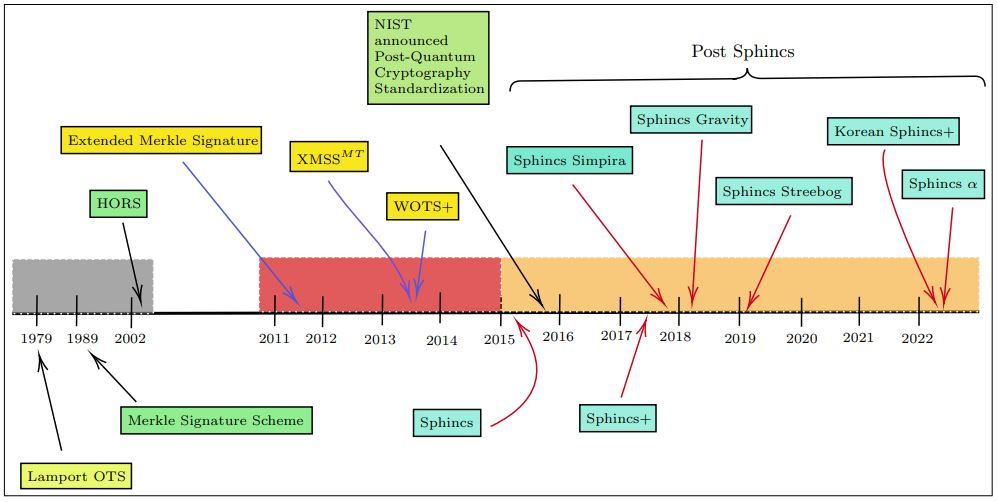
\includegraphics[scale=0.6]{images/timeline.jpg}
\caption{Хронология развития алгоритмов ЭЦП на основе хэш-функций \cite{timeline}}
\end{figure}

\subsubsection{SPHINCS$^+$}

SPHINCS$^+$ -- это алгоритм ЭЦП на основе хэш-функции, выбранный в качестве финалиста второго раунда конкурса стандартизации алгоритмов постквантовой криптографии от NIST. 

 Введем несколько понятий, используемых в аппарате алгоритма SPHINCS+.

\textbf{Определение.} Гипердерево -- это дерево многоразовых подписей на основе хэш-функции.

\textbf{Определение.} Хэш-дерево -- это полное двоичное дерево, в листовые вершины которого помещены хэши от блоков данных, внутренние вершины содержат хэши от сложения значений в дочерних вершинах, а корневой узел дерева содержит хэш от всего набора данных.


Схема SPHINCS+ использует гипердерево Меркла, состоящее из множества бинарных хэш-деревьев, которые соединены между собой одноразовой схемой подписи (Winternitz-type OTS) WOTS$^+$. Открытый ключ хранится в корне гипердерева. В нижней части гипердерева используется малократная подпись (Forest of Random Subsets) FORS.

Например, гипердерево схемы подписи SPHINCS$^+$ можно изобразить следующим образом:

\begin{figure}[H]
\centering
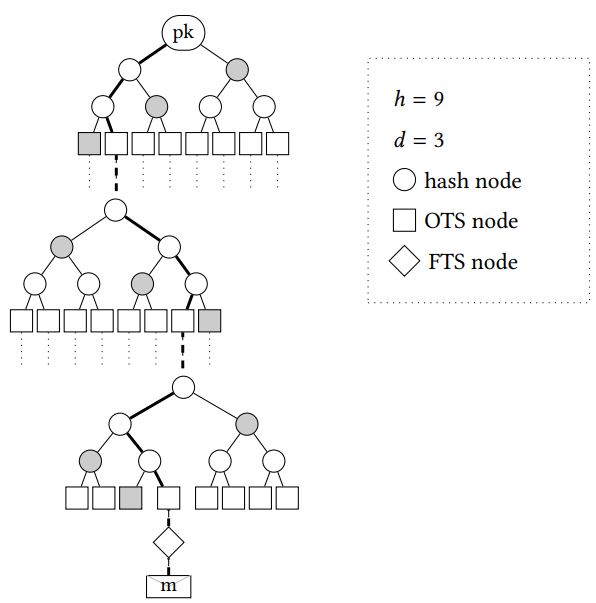
\includegraphics[scale=0.8]{images/sphincs+.JPG}
\caption{Cхема алгоритма SPHINCS$^+$ \cite{sphincs_scheme}}
\end{figure}

\textbf{Достоинства и недостатки алгоритма SPHINCS$^+$ }\cite{doc_sphincs}

Недостаток: размер подписи и скорость.

Достоинства: 
\begin{itemize}
\item 
безопасность SPHINCS$^+$ основана на
предположениях о безопасности используемой хэш-функции;
\item
наиболее эффективные известные атаки против SPHINCS$^+$ легко установить и проанализировать;
\item
небольшой размер ключей, в частности размер открытого ключа (несомненное преимущество при частой передаче сертификатов, например, SSL/TLS).
\end{itemize}
\clearpage
\section{Заключение}

На данном этапе развития постквантовых криптографических алгоритмов сложно отдать предпочтение какому либо из них. В то время как одни предстают в лучшем свете с точки зрения размеров ключей, другие базируются на математических задачах, считающихся на данный момент более полно изученными, а значит надёжными в долгосрочной перспективе.

В с связи с вышеупомянутыми фактами, данная область криптографии нуждается в более глубоком анализе существующих решений, их тестировании и сравнении.

\clearpage

%\section{Список использованных источников информации}

%\clearpage

%\section{Приложения}
\clearpage

%\newrefcontext[sorting=ntvy]
%\printbibliography[env=gostbibliography]
%\addcontentsline{toc}{chapter}{bibname}
\renewcommand{\refname}{Список использованных источников информации}
\addcontentsline{toc}{section}{Список использованных источников информации}
%\bibliographystyle{gost780s}
%\bibliographystyle{utf8gost705u}
\bibliographystyle{unsrt}
\bibliography{refs}{}
\end{document}